\section{Termodinâmica}\label{sec:LABEL_CHP_2_SEC_A}

\subsection{Equilíbrio Termodinâmico}\label{sec:LABEL_CHP_2_SEC_A_SUB_A}


Uma parte de um sistema em que as propriedades e composição são homogêneas, e que é fisicamente distinta de outras partes do mesmo sistema pode ser definida como uma fase. Em um sistema composto por uma ou mais fases, o que diferencia cada parte deste sistema são seus componentes, isto é, diferentes elementos ou compostos químicos que constituem o sistema, assim como a composição de cada fase deste sistema pode ser definida como diferentes grupos de cada componente \cite{porter2009phase}.

Em um sistema com diferentes fases, elementos ou compostos químicos, é esperado que cada elemento tenha uma interação com os elementos que o rodeiam. Para um sistema ser considerado estável ou instável diversos fatores devem ser levados em conta, essa estabilidade relativa é estimada através da energia de livre de Gibbs, essa grandeza é determinada através da entalpia, entropia e da temperatura.

A energia livre de Gibbs de um sistema em que temos temperatura e pressão constantes, é dada pela Equação \ref{eq:gibbs}.

\begin{equation} 
G = H - TS
\label{eq:gibbs}
\end{equation}

Onde H é a entalpia, S é a entropia e T é a temperatura absoluta (K). Resumidamente temos que:

\begin{itemize}
  \item Quando $\Delta G < 0$ o processo é exergônico, ocorrerá de forma espontânea a formação de mais produtos.
  \item Quando $\Delta G > 0$ o processo é endergônico, ocorrerá de forma espontânea a formação de mais reagentes.
  \item Quando $\Delta G = 0$ o sistema está em equilíbrio e a concentração de produtos e reagentes permanecerão constantes. \cite{gaskell2012introduction}
\end{itemize}

\begin{table}[htb]
\centering
\caption{Espontaneidade quando $\Delta G < 0$ }
\begin{supertabular}{|m{2.0cm}|m{4.5cm}|m{4.5cm}|}
\hline
{  } &
{ $\Delta H < 0$ } &
{ $\Delta H > 0$ }\\\hline
{ $\Delta S > 0$ } &
{ Espontânea para todas T
( $\Delta G < 0$) } &
{ Espontânea para altas T
(quando $ T\Delta S$ é grande)
} \\\hline
{ $\Delta S < 0$ } &
{ Espontânea para baixas T
(quando $ T\Delta S$ é pequeno) } &
{ Não Espontânea para todas T
( $\Delta G > 0$) } \\\hline
\end{supertabular}
    \legend{}
    \label{quad:espontaneidade}
\end{table}

Considerando um sistema composto por átomos A e B em solução sólida. Cada átomo possui a sua respectiva energia livre de Gibbs, sendo assim ao considerar um sistema homogêneo em solução sólida dos elementos A e B, e que estes possuem a mesma estrutura cristalina, temos a energia livre de Gibbs deste sistema dada pela Equação \ref{eq:ss-mistura}:

\begin{equation} 
G = X_{A}G_{A} + X_{B}G_{B} + \Delta G_{mix}
\label{eq:ss-mistura}
\end{equation}

Onde $X_{A}$ e $X_{B}$ são as frações molares dos elementos A e B, $G_{A}$ e $G_{B}$ são as energias livres de Gibbs dos elementos A e B puros e $\Delta G_{mix}$ é a variação na energia livre de Gibbs devido à mistura dos átomos. Essa variável é determinada através da Equação \ref{eq:deltaG-mix}:

\begin{equation} 
\Delta G_{mix} = \Delta H_{mix} - T\Delta S_{mix}
\label{eq:deltaG-mix}
\end{equation}

Onde $\Delta H_{mix}$ é o calor envolvido durante a mistura dos elementos e $\Delta S_{mix}$ é a variação de entropia provocada pela mistura.

A entropia de uma solução sólida na termodinâmica estatística é quantificada através da aleatoriedade dada através da Equação \ref{eq:entropia-boltzmann}. Onde k é a constante de Boltzmann e $\omega$ é a medida de aleatoriedade. Essa entropia possui duas contribuições significativas, a contribuição térmica  e a contribuição configuracional. No caso da entropia térmica, a medida de aleatoriedade é dada pela quantidade de formas que a energia térmica de um sólido pode ser dividida entre os átomos, que é, a quantidade total de estados vibracionais de um sólido. Em soluções, devido as diferentes formas que os átomos podem ser arranjados existem também uma aleatoriedade adicional, isto nos leva a entropia configuracional, isto é, a o total de formas distintas em que os átomos de uma solução podem se organizar.

\begin{equation} 
 S =  k\ln \omega
\label{eq:entropia-boltzmann}
\end{equation}

Quando a variação de volume ou troca de calor durante a mistura é zero, a única contribuição para a entropia de mistura $\Delta S_{mix}$ será a entropia configuracional. 
\begin{equation} 
\omega_{config}=\frac{(N_{A} + N_{B})!}{N_{A}!N_{B}!}
\label{eq:entropia-config}
\end{equation}

Onde $N_{A}$ é a quantidade de átomos de A e $N_{B}$ a quantidade de átomos de B respectivamente. Uma vez que está sendo considerada uma solução de 1 mol, isto é, $N_{a}$ átomos (número de Avogadro), temos 
$N_{A}= X_{A}N_{a}$ e $N_{B}= X_{B}N_{a}$. Substituindo as equações (\ref{eq:entropia-boltzmann}) e (\ref{eq:entropia-config}) e usando a aproximação de Stirling ($\ln N! \simeq N \ln N - N$) e o relacionamento $N_{ak} = R$ (a constante universal dos gases) temos a entropia de mistura de uma solução sólida binária na Equação \ref{eq:entropia-mix} :

\begin{equation} 
\Delta S_{mix} = -R(X_{A}\ln X_{A} + X_{B}\ln X_{B})
\label{eq:entropia-mix}
\end{equation}


Uma vez que  $X_{A}$ e $X_{B}$ são valores menores que um, podemos concluir que há sempre um aumento na entropia do sistema devido à mistura dos elementos.

\subsection{Soluções Ideais}\label{sec:LABEL_CHP_2_SEC_A_SUB_B}

 A forma mais simples de mistura para de início é quando temos $\Delta H_{mix}=0$, consequentemente, segundo as Equações \ref{eq:deltaG-mix} e \ref{eq:entropia-mix}, temos a energia livre de Gibbs   \ref{eq:delta-gibbs}.

\begin{equation} 
\Delta G_{mix} = RT(X_{A}\ln X_{A} + X_{B}\ln X_{B})
\label{eq:delta-gibbs}
\end{equation}

Dessa forma, à partir das Equações \ref{eq:ss-mistura} e \ref{eq:delta-gibbs}, a energia livre de Gibbs do sistema pode ser definida pela Equação \ref{eq:livre-gibbs}:

\begin{equation} 
G=X_{A}G_{A} + X_{B}G_{B} + RT(X_{A}\ln X_{A} + X_{B}\ln X_{B})
\label{eq:livre-gibbs}
\end{equation}

Os valores de energia livre de Gibbs em função da variação de composição e
temperatura estão esquematizados na Figura \ref{fig:energia-livre-gibbs}, pode-se notar que para altas temperaturas, $G_{A}$ e $G_{B}$ ocorre uma redução significativa na energia livre de Gibbs de um sistema.

\begin{figure}[ht]
    \centering
    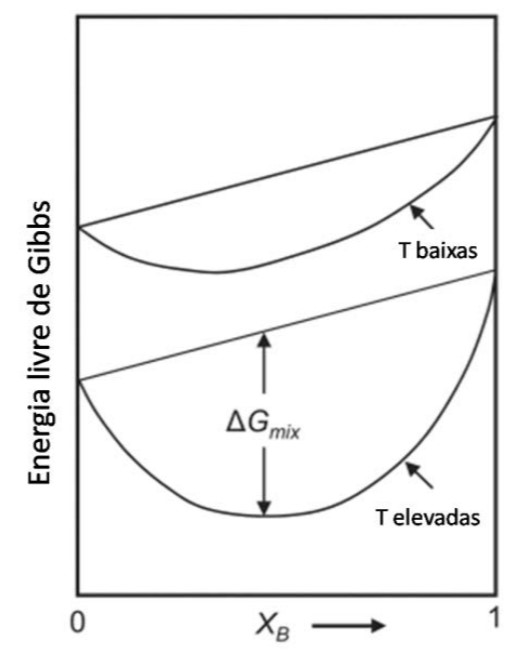
\includegraphics[height=7.5cm]{energia-livre-gibbs.jpg} 
    \caption{Energia livre de Gibbs de uma solução ideal. Adaptado de \cite{porter2009phase}.}
    \label{fig:energia-livre-gibbs}
\end{figure}

\subsection{Soluções Regulares}\label{sec:LABEL_CHP_2_SEC_A_SUB_C}

Analisando uma forma de mistura em que diferente do modelo ideal onde $\Delta H = 0$, temos um comportamento de contribuição da entalpia ($\Delta H \neq 0$) na energia livre de Gibbs, que na prática podemos observar uma mistura endotérmica (calor absorvido $\Delta H_{mix}>0$), ou uma mistura exotérmica (calor liberado $\Delta H_{mix}<0$). Novamente considerando os átomos A e B apresentando a as estruturas semelhantes, e que não a variação do volume durante a mistura, a entalpia de mistura será apenas função das energias de ligação entre os átomos adjacentes. Podemos considerar três possíveis energias de ligação neste modelo:
\begin{itemize}
  \item Ligações A--A, cada um com a energia $ \varepsilon_{AA}$, 
  \item Ligações B--B, cada um com a energia $ \varepsilon_{BB}$,
  \item Ligações A--B, cada um com a energia $ \varepsilon_{AB}$,
\end{itemize}

\begin{figure}[ht]
    \centering
    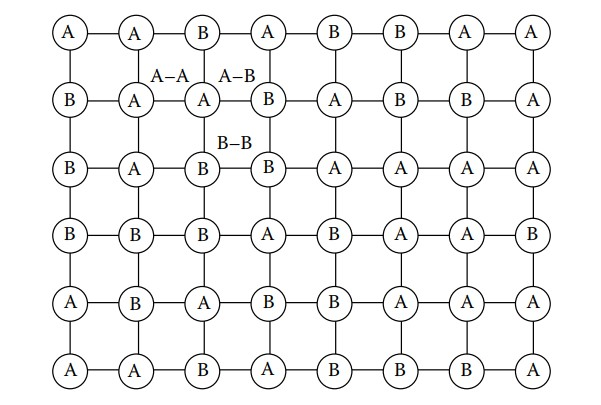
\includegraphics[height=7cm]{ligacoes.jpg} 
    \caption{Os diferentes tipos de ligações interatômicas em uma solução sólida. Adaptado de \cite{porter2009phase}.}
    \label{fig:ligacoes-interatomicas}
\end{figure}

A energia interna da solução E irá depender do número de ligações para cada tipo $P_{AA}$, $P_{BB}$ e $P_{AB}$: 
\begin{equation} 
E = P_{AA}\varepsilon_{AA} +  P_{BB}\varepsilon_{BB} + P_{AB}\varepsilon_{AB}
\label{eq:energia-interna-solucao}
\end{equation}
b
Antes de misturar, os elementos A e B puro, contém respectivamente as ligações A--A e B--B, e considerando a relação entre $P_{AA}$, $P_{BB}$ e $P_{AB}$, a mudança na energia interna da mistura é dada pela Equação \ref{eq:entalpia-ligacao}.
\begin{equation} 
\Delta H_{mix} = P_{AB} \varepsilon
\label{eq:entalpia-ligacao}
\end{equation}
Onde:
\begin{equation} 
\varepsilon = \varepsilon_{AB} - \frac{1}{2} ( \varepsilon_{AA} + \varepsilon_{BB})
\label{eq:energia-ligacao}
\end{equation}

Ou seja, $\varepsilon$ é a diferença entre a energia de ligação A--B e a média entre as energias de ligação de A--A e B--B. Sendo assim, se $\varepsilon=0$, $\Delta H_{mix}=0$ o que nos leva a solução ideal. No caso em que os átomos estão arranjados completamente aleatórios e a entropia de mistura é dada pela Equação \ref{eq:entropia-mix}. Então pode ser demostrado que:

\begin{equation} 
P_{AB} = N_{a}z X_{A}X_{B} \textrm{  ligações.mol}^{-1} 
\label{eq:energia-AB}
\end{equation}

Onde $N_a$ é o número de Avogadro e $z$ é o número de ligações por átomo. Se $\varepsilon<0$ os átomos na solução irão dar preferência a fazer ligações com o átomo oposto, resultando no aumento de $P_{AB}$, enquanto que, se $\varepsilon>0$, $P_{AB}$ será menor do que numa solução aleatória. Considerando que $\varepsilon$ não é tão diferente de zero, podemos reescrever a Equação \ref{eq:energia-AB}:

\begin{equation} 
\Delta H_{mix} = \Omega X_{A}X_{B}
\label{eq:entalpia-mistura}
\end{equation}

Onde:

\begin{equation} 
\Omega = N_{a}z \varepsilon
\label{eq:omega}
\end{equation}

Sendo assim podemos determinar os valores da energia livre de Gibbs em função de $\Omega$ e da temperatura, substituindo a Equação \ref{eq:deltaG-mix} por  \ref{eq:entropia-mix} e  \ref{eq:entalpia-mistura} temos que:

\begin{equation} 
\Delta G_{mix} = \Omega X_{A}X_{B} + RT(X_{A}\ln X_{A} + X_{B}\ln X_{B})
\label{eq:deltaG-mix-regular}
\end{equation}


A equação \ref{eq:deltaG-mix-regular} pode ser representada na figura \ref{fig:gibbs-temperatura-composicao}, em diferentes valores de $\Omega$ e de temperatura, temos diferentes comportamentos na entropia e entalpia e consequentemente alterando a energia livre de Gibbs. 

\begin{figure}[ht]
    \centering
    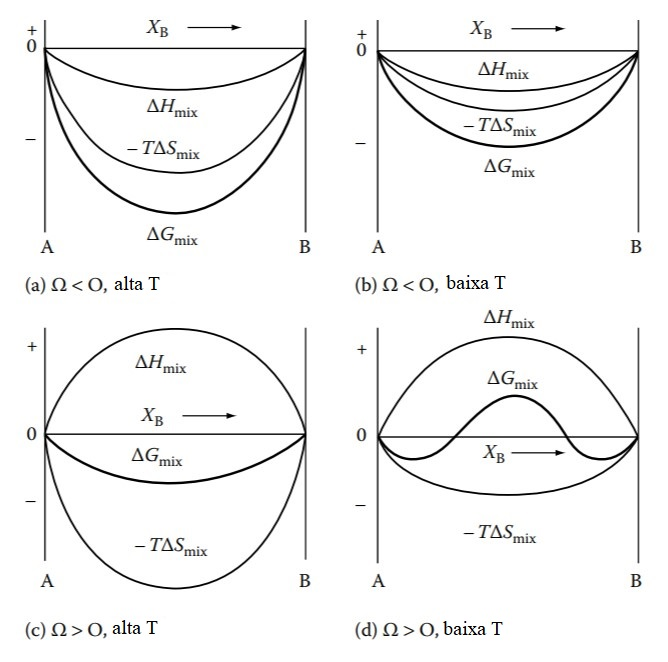
\includegraphics[height=12cm]{gibbs-temperatura-composicao2.jpg} 
    \caption{Resultado da influência da temperatura, composição e número de ligações nos valores da energia de Gibbs, entalpia e entropia. Adaptado de \cite{porter2009phase}.}
    \label{fig:gibbs-temperatura-composicao}
\end{figure}

\pagebreak

De acordo com a Figura \ref{fig:gibbs-temperatura-composicao} é observado que quando a composição $X_{A}$ e $X_{B}$ são iguais, isto é, quando a composição se torna equiatômica, a energia livre de Gibbs atinge seu menor valor. Consequentemente em ligas com composição equiatômica quando em solução sólida, tendem a apresentar fases estáveis, possibilitando uma composição de fase homogênea do material produzido.

Em um cenário ideal a confecção de ligas com a composição equiatômica, possibilitaria desenvolver um material com propriedades significativamente superiores aos materiais de ligas convencionais de uma matriz com elemento dominante. Porém a explicação abordada anteriormente se refere a um caso simples com apenas dois elementos. Ao se tratar de uma liga mais complexa com cinco ou mais elementos, os parâmetros para definição da energia livre de Gibbs se tornam mais complexos, e quando a entalpia de mistura é diferente de zero, nem sempre o equiatomicidade resultará na menor energia livre de Gibbs, isto devido a interferência da energia de ligação interatômica. Neste caso quando é observado um comportamento em que a energia de ligação supera a energia livre de Gibbs  há a formação de compostos intermetálicos \cite{porter2009phase}.
